\section{Architektura}
Architektura aplikace je členěna do tří balíků reprezentujících logicky odlišné funkční celky. Hierarchie balíků je znázorněna na diagramu \emph{\ref{diagram-bundles}}.

\begin{figure}[htbp]
    \centering
    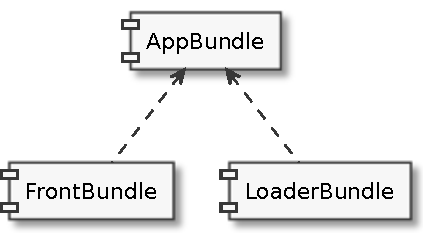
\includegraphics[width=0.5\textwidth,height=\textheight,keepaspectratio]{pdfs/bundles}
    \caption{Architektura komponent\label{diagram-bundles}}
\end{figure}

\paragraph{AppBundle}  
je základním balíkem aplikace obsahujícím implementaci datové vrstvy aplikace, zodpovědné za persistenci dat a jejich zpřístupnění. Dále obsahuje implementaci klienta pro přístup k~datům Brickset přes API a implementaci business logiky aplikace.

\paragraph{FrontBundle} 
obsahuje implementaci uživatelského rozhraní aplikace v~podobě \textit{Controller} tříd a \textit{Twig} šablon sloužících k~zobrazení dat uživateli.

\paragraph{LoaderBundle} 
zastřešuje logiku aplikace pro načítání součástek knihovny LDraw a databáze Rebrickable z~\gls{CSV} souborů za pomoci konzolových příkazů \autocite{symfony:console}. 

